\subsection{Электрические цепи постоянного тока. ЭДС. Правила Кирхгофа}

\begin{definition}
    Электрическая цепь постоянно тока — совокупность устройств и объектов: источников электрической энергии, 
    преобразователей, потребителей, коммутационной, защитной и измерительной аппаратуры, соединительных проводов 
    или линии электропередачи.

    Электрические и электромагнитные процессы в этих объектах описываются с помощью понятий об электродвижущей 
    силе (ЭДС), токе ($I$) и напряжении ($U$).
\end{definition}

\begin{remark}
    Для существования постоянного тока необходимо наличие в электрической цепи устройства, способного создавать и 
    поддерживать разности потенциалов на участках цепи за счет работы сил неэлектростатического происхождения. 
    Такие устройства называются источниками постоянного тока
\end{remark}

Силы неэлектростатического происхождения, действующие на свободные носители заряда со стороны источников тока, 
называются сторонними силами.

Сторонние силы характеризуются своей работой над зарядом.

\begin{definition}
    Электродвижующая сила источника (ЭДС) $[\varepsilon,\ В]$ — физическая величина, равная отношению работы $A_{ст}$ сторонних сил при перемещении заряда $q$ от отрицательного полюса источника тока к положительному к величине этого заряда:

    $$
    \varepsilon=\frac{A}{q}
    $$
\end{definition}

Стороннюю силу можно представить в виде:

$$
\vec F_{стор}=\vec E_{стор}\ q
$$

где $E_{стор}$ - напряженность поля сторонних сил

\begin{definition}
    Работа сторонних сил над зарядом на участке цепи $1-2$:

    $$
    A_{12}=\int_1^2(\vec F_{стор},\ d\vec l)=q\int_1^2(\vec E_{стор},\ d\vec l)
    $$
\end{definition}

По определению электродвижущей силы:

$$
\varepsilon=\int_1^2(\vec E_{стор},\ d\vec l)
$$

Для замкнутой цепи ЭДС равна циркуляции напряженности поля сторонних сил:

$$
\varepsilon=\oint(\vec E_{стор},\ d\vec l)
$$

Разветвленные цепи. Правила Кирхгофа.

\begin{definition}
    Первое правило Кирхгофа.

    Узел — точка, в которой сходятся три и более проводника.
\end{definition}

Узел не может накапливать заряды: алгебраическая сумма токов, сходящихся в узле, равна 0:
$$
\sum_iI_i=0
$$

Токи, входящие в узел, считаются положительными, а вытекающие — отрицательными.

При расчётах цепей, уравнений такого типа записывается на одно меньше, чем насчитывается узлов в цепи. 
Если число уравнений соответствует числу узлов, то одно из них является следствием из всех остальных, что только загромождает расчеты. 

\begin{definition}
    Второе правило Кирхгофа.

    В любом замкнутом контуре разветвленной электрической цепи алгебраическая сумма ЭДС, действующих в этом контуре, равна сумме произведений токов в каждой его ветви на их сопротивления:

    $$
    \sum_{i=1}^n\varepsilon_i=\sum_{i=1}^nI_iR_i
    $$

    где $n$ — число участков, на которые контур разбивается узлами
\end{definition}

\begin{figure}[h]
    \centering
    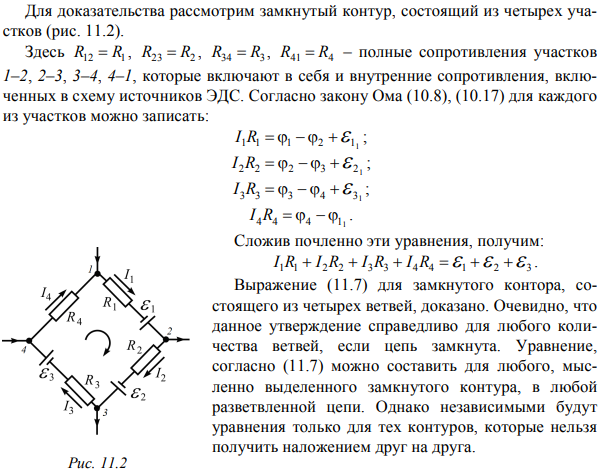
\includegraphics[width=0.5\linewidth]{imgs/q33i1.png}
\end{figure}

\begin{figure}[h]
    \centering
    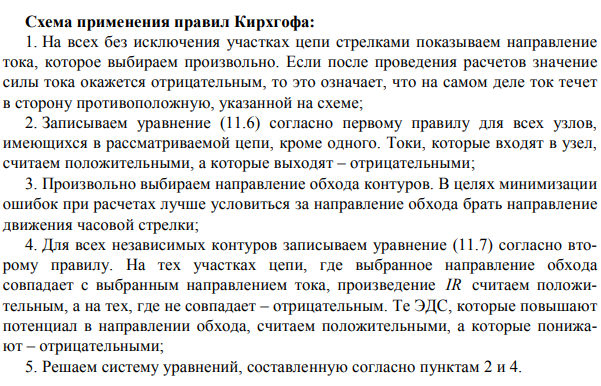
\includegraphics[width=0.5\linewidth]{imgs/q33i2.png}
\end{figure}